% !TEX TS-program = xelatex
% !TEX encoding = UTF-8 Unicode
% !Mode:: "TeX:UTF-8"
\documentclass[bachelor,nocolorlinks, printoneside]{seuthesis} % 本科
% \documentclass[master]{seuthesis} % 硕士
% \documentclass[doctor]{seuthesis} % 博士
% \documentclass[engineering]{seuthesis} % 工程硕士
\usepackage{CJK,CJKnumb}
\usepackage{amsmath}
\usepackage{amsfonts} 
\usepackage{bm} 
\usepackage{algorithm}
\usepackage{algorithmicx}
\usepackage{algpseudocode}
\usepackage{subfigure}
\usepackage{booktabs}
\usepackage{appendix}
\usepackage{listings}
\usepackage{ctex}
% 用来设置附录中代码的样式
\lstset{
    basicstyle          =   \sffamily,          % 基本代码风格
    keywordstyle        =   \bfseries,          % 关键字风格
    commentstyle        =   \rmfamily\itshape,  % 注释的风格,斜体
    stringstyle         =   \ttfamily,  % 字符串风格
    flexiblecolumns,                % 别问为什么,加上这个
    numbers             =   left,   % 行号的位置在左边
    showspaces          =   false,  % 是否显示空格,显示了有点乱,所以不现实了
    numberstyle         =   \zihao{-5}\ttfamily,    % 行号的样式,小五号,tt等宽字体
    showstringspaces    =   false,
    captionpos          =   t,      % 这段代码的名字所呈现的位置,t指的是top上面
    frame               =   lrtb,   % 显示边框
}

\lstdefinestyle{C++}{
    language        =   C++, % 语言选Python
    basicstyle      =   \zihao{-5}\ttfamily,
    numberstyle     =   \zihao{-5}\ttfamily,
    keywordstyle    =   \color{blue},
    keywordstyle    =   [2] \color{teal},
    stringstyle     =   \color{magenta},
    commentstyle    =   \color{red}\ttfamily,
    breaklines      =   true,   % 自动换行,建议不要写太长的行
    columns         =   fixed,  % 如果不加这一句,字间距就不固定,很丑,必须加
    basewidth       =   0.5em,
}
%%xiaoxiao
\usepackage{titlesec}
\usepackage{titletoc}
\setcounter{tocdepth}{1}
\setcounter{secnumdepth}{1}
%%xiaoxiao


\floatname{algorithm}{算法}
\renewcommand{\algorithmicrequire}{\textbf{输入:}}
\renewcommand{\algorithmicensure}{\textbf{输出:}}
 % 这里是导言区

\begin{document}
\categorynumber{000} % 分类采用《中国图书资料分类法》
\UDC{000}            %《国际十进分类法UDC》的类号
\secretlevel{公开}    %学位论文密级分为"公开"、"内部"、"秘密"和"机密"四种
\studentid{你的学号}   %学号要完整,前面的零不能省略。

\title{论文题目}{}{title}{subtitle}
\author{你的名字}{your name}
\advisor{导师名字}{导师职称}{导师名字英文}{Associate Prof.}
\coadvisor{校内导师名字}{导师职称}{导师名字英文}{Associate Prof.} % 没有

% \degree{工学硕士} % 详细学位名称
\major[12em]{专业}
\defenddate{答辩日期}
\authorizedate{学位授予日期}
\department{软件}{department name}
\duration{毕设起止日期}
\address{}
\thanks{}
\maketitle

%%xiaoxiao
\titleformat*{\chapter}{\bfseries\center\sanhao\hei}
\titleformat*{\section}{\sihao\hei}
\titleformat*{\subsection}{\xiaosihao\song}
%%xiaoxiao
\begin{abstract}{关键字}
这里是中文摘要
\end{abstract}

\begin{englishabstract}{key word}
英文摘要
\end{englishabstract}

\tableofcontents

\begin{Main} % 开始正文

\chapter{数学公式}
\emph{这里可以写点东西}
\section{行内数学公式}
这是一段话,包含了一个行内公式
$\sum_{t=1}^{T}{k_t} = \frac{1}{2} \gamma$
\section{数学公式}
这是一个普通的数学公式
\begin{equation}q_{\pi}(s,a)=\mathcal{R}^a_{s}+\gamma\sum_{s^{\prime}\in S}{\mathcal{P}^a_{ss^{\prime}}\sum_{a^{\prime}\in A}\pi(a^{\prime}|s^{\prime})q_{\pi}(a^{\prime},s^{\prime})}
\end{equation}

\section{带有大括号的数学公式}
这是一个带有大括号的数学公式
\begin{equation}
p_{ij}^{k}=\\
\left\{
    \begin{array}{lr}
    \frac{{\lbrack \tau_{ij}(t)\rbrack}^{\alpha}{\lbrack \eta_{ij}\rbrack}^{\beta}}{\sum_{k \in A}{{\lbrack \tau_{ik}(t)\rbrack}^{\alpha}{\lbrack \eta_{ik}\rbrack}^{\beta}} }  &  k \in Available\\
    0 &else
    \end{array}
\right.
\end{equation}

\chapter{图片}
\section{普通图片}
\begin{figure}[htbp!]
    \centering 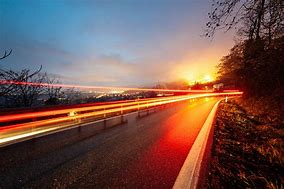
\includegraphics[width=0.6\textwidth]{img/1.jpg} \caption{测试图片}
\end{figure}

\section{子图}
\begin{figure}
    \centering
    \subfigure[测试图片1]{
    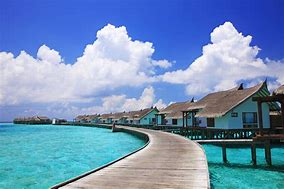
\includegraphics[width=0.4\textwidth]{img/2.jpg} 
    }
    \subfigure[测试图片2]{
    
\includegraphics[width=0.4\textwidth]{img/3.jpg} 
    }
    \subfigure[测试图片3]{
    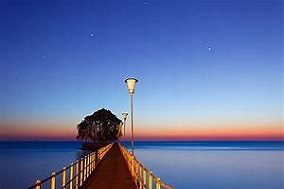
\includegraphics[width=0.4\textwidth]{img/4.jpg} 
    }
    \subfigure[测试图片4]{
    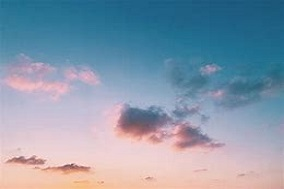
\includegraphics[width=0.4\textwidth]{img/5.jpg} 
    }
    \caption{带有子图的图片}
\end{figure}


\chapter{算法}
\begin{algorithm}
    \caption{ACO算法解决TSP}
    \begin{algorithmic}[1] %每行显示行号
        \Require 图$G(V,E)$,$d_{ij}$城市$i$与城市$j$的距离,蚂蚁的集合$M$
        \Ensure 最短路径,最短路径的长度
        \Function{constructRoutes}{}
            \For{$i$ in $1,\cdots,|V|-1$}
                \For{$\forall k \in M$}
                    \State 选择下一个城市$s_k$
                    \State 增加边$edge(r_k,s_k)$
                    \State $r_k \leftarrow s_k$
                \EndFor
            \EndFor
            \For{$\forall k \in M$}
                \State 增加边$edge(r_k,s_k)$
            \EndFor
        \EndFunction
        \Function{updatePheromones}{}
            \For{$\forall k \in M$}
                \State 计算$L_k$
                \State 更新$\tau_{r,s}$
            \EndFor
        \EndFunction
        \Function{main}{}
            \For{$\forall dege(r,s) \in E$}
                \State $\tau_{r,s} \leftarrow \tau_0$
                \State $\eta_{r,s} \leftarrow \frac{1}{c_{r,s}}$
            \EndFor
            \While{结束条件不满足}  
                \State 调用setInitInfo函数
                \State 调用constructRoutes函数
                \State 调用updatePheromones函数
            \EndWhile
        \EndFunction
    \end{algorithmic}
\end{algorithm}

\chapter{列表}
\section{有序列表}
\begin{enumerate}[(1)]
    \item 随便说点东西
    \item 随便说点东西
    \item 随便说点东西
\end{enumerate}

\section{无序列表}
\begin{enumerate}[$\cdot$]
    \item 随便说点东西
    \item 随便说点东西
    \item 随便说点东西
\end{enumerate}

\chapter{表格}
以下是一个论文中常用的三线表的格式,其中{tabular}{cccccc},其中每一个l表示居左r表示居右c表示居中,其中用p表示每列的宽度,例如cp5em,表示居中列宽5em
\begin{table}[htbp]
    \centering
    \caption{年龄与工作,房子有无,信贷关系数据表}
      \begin{tabular}{cccccc}
      \toprule
      ID       & 年龄段      & 有工作      & 有自己的房子   & 信贷情况     & 类别(是否给贷款) \\
      \midrule
      1        & 青年       & 否        & 否        & 一般       & 否 \\
      2        & 青年       & 否        & 否        & 好        & 否 \\
      3        & 青年       & 是        & 否        & 好        & 是 \\
      4        & 青年       & 是        & 是        & 一般       & 是 \\
      ...      & ...      & ...      & ...      & ...      & ... \\
      498      & 老年       & 是        & 否        & 非常好      & 是 \\
      499      & 老年       & 否        & 否        & 一般       & 否 \\
      500      & 老年       & 否        & 否        & 非常好      & 否 \\
      \bottomrule
      \end{tabular}%
    \label{tab:addlabel}%
\end{table}%

\chapter{论文引用}
这是一段比较有趣的话\cite{ref1},因为在这短短的一段文字中,居然有两个引用\cite{ref2}

论文引用可以使用bibtex或者使用zotero集体导出GB/T 7714-2015格式的引用

zotero导出论文引用时,将所有引用论文添加到一个单独拿的文件夹中,右键选择“由所选条目创建引文条目”->“引文目录”,“复制到剪贴板”

\end{Main} % 结束正文

% 参考文献
\bibliography{seuthesis}
\begin{thebibliography}{99}  
    \bibitem{ref1}王亚杰, 邱虹坤, 吴燕燕, 等. 计算机博弈的研究与发展[J]. 智能系统学报, 2016, 11(6): 788-798.
    \bibitem{ref2}徐心和, 邓志立, 王骄, 等. 机器博弈研究面临的各种挑战[J]. 智能系统学报, 2008(04): 288-293.
\end{thebibliography}


%附录A
\begin{appendices}
    \renewcommand{\thechapter}{\Alph{chapter}.}
    \chapter*{附录 A}
    随便写点东西
    \chapter*{附录 B}
    \section*{标题}
    \lstinputlisting[
    style       =   C++,
    caption     =   {\bf Kmeans.py},
    label       =   {Kmeans.py}
]{D:/programFiles/vscode/seuthesis-2.5.3/img/Kmeans.py}
\end{appendices}

%致谢
\begin{Acknowledgement}{}
感谢大家
\end{Acknowledgement}

\newpage
\printindex % 索引

%\begin{thebibliography}{99}
%\bibliographystyle{ieee}
%\bibliography{seuthesis}

\end{document}
